\section{\deleted{Approximate transparent boundary conditions for the dispersion equation} \added{Interfac boundary condition operators based on the exact TBCs for the dispersion equation}}
\label{sec:TBC}

\subsection{The exact TBCs for the continuous equation}

\indent In \cite{besse2015}, transparent boundary conditions (TBCs) are derived for the one-dimensional continuous linearized KdV equation (or Airy equation):

\begin{equation}
 	\label{eq:LKdV}
 	u_t + U_1u_x + U_2u_{xxx} = h(t,x), \ \ t \in \mathbb{R}^+, \ \ x \in \mathbb{R}
\end{equation}

\noindent where $U_1 \in \mathbb{R}$, $U_2 \in \mathbb{R}^+_*$ and $h$ is a source term, assumed to be compactly supported in a finite computational domain $[a,b], \ a < b$.

\indent For the homogeneous initial boundary value problem 

\begin{equation*}
\begin{cases}
	u_t + U_1u_x + U_2u_{xxx} = 0, \ \ t \in \mathbb{R}^+, \ \ x \in [a,b] \\
	u(0,x) = u_0(x), \ \ x \in [a,b] \\
	+ \text{boundary conditions} \nonumber
\end{cases}
\end{equation*}

\noindent the TBCs are given \cite[equations (2.17) -(2.18)]{besse2015} by 

\begin{equation}
\label{eq:continuousTBC}
\begin{gathered}
        u(t,a) - U_2 \laplinv \left( \frac{\lambda_1(s)^2}{s} \right) * u_x(t,a) - U_2 \laplinv \left( \frac{\lambda_1(s)}{s} \right) * u_{xx}(t,a) = 0 \\ 
        u(t,b) - \laplinv \left( \frac{1}{\lambda_1(s)^2} \right) * u_{xx}(t,b) = 0 \\
        u_x(t,b) - \laplinv \left( \frac{1}{\lambda_1(s)} \right) * u_{xx}(t,b) = 0 
\end{gathered}
\end{equation}

\noindent where $\laplinv$ denotes the inverse Laplace transform, $*$ the convolution operator, $s \in \mathbb{C}, \ Re(s)>0$ is the Laplace frequency and $\lambda_1$ is, among the three roots of the cubic characteristic equation obtained when solving \eqref{eq:LKdV} in the Laplace space and in the complementary set of $[a,b]$, the only one with negative real part.

\indent In this paper, we will focus on the special case $U_1 = 0, U_2 = 1$, which results on the dispersion equation \eqref{eq:DKdV}. In this case, accordingly to \cite{zheng2008}, the only root with negative real part is 

\begin{equation}
	\label{eq:lambda}
			\lambda(s) = \lambda_1(s) =  -\sqrt[3]{s} 
\end{equation}

\subsection{\deleted{Approximation of the TBCs} \added{Construction of operators based on the exact TBCs}}

\indent The computation of the TBCs \eqref{eq:continuousTBC} is not simple due to the inverse Laplace transform, which makes these conditions nonlocal in time. Therefore, we will propose approximations of the root \eqref{eq:lambda} that avoid integrations in time, making the \deleted{TBCs} \added{operators} considerably simpler.

\indent Obviously, as we can see through the results shown in this section, \deleted{the approximate boundary conditions are not as accurate as the ones}\added{when playing the role of transparent boundary conditions, these operators are not as accurate as the approximate TBCs} proposed by \cite{besse2015} (who derives TBCs for the discrete linearized KdV equation). Nevertheless, the objectives of our work and the work of \cite{besse2015} are very different: while they seek to minimize the error of the computed solution (compared to the analytical one) due to the boundary conditions, we want here to apply our \deleted{approximate TBCs} \added{operators} as interface boundary conditions (IBCs) in a domain decomposition method (DDM). Therefore, our objective lays on the convergence of the DDM to the solution of the same problem in the monodomain, independently of the errors on the external boundaries. 

\indent We will use the constant polynomial $P_0(s) = c$ for approximating $\lambda^2/s$. Moreover, as a consequence of \eqref{eq:lambda}, we can approximate the other operands of the inverse Laplace transforms in \eqref{eq:continuousTBC} only in function of $c$ :

\begin{equation}
	\label{eq:appP0}
	\frac{\lambda^2}{s}  = c, \qquad
	\frac{\lambda}{s}  = -c^2, \qquad
	\frac{1}{\lambda(s)^2}  = c^2, \qquad 
	 \frac{1}{\lambda(s)}  = -c 
\end{equation}

\indent Replacing \eqref{eq:appP0} in \eqref{eq:continuousTBC}, using some well-know properties of the Laplace Transform (linearity and convolution) and considering possibly different polynomial approximations for the left and the right boundaries (respectively with the coefficients $c_L$ and $c_R$), we get the approximate transparent boundary conditions

%\begin{equation}
%\label{eq:appTBCP0}
%    \begin{cases}
%        u(t,a) - c u_x(t,a)  + c^2  u_{xx}(t,x) = 0 \\
%        u(t,b) - c^2    u_{xx}(t,x) = 0 \\
%        u_x(t,b) + c u_{xx}(t,x)= 0 
%    \end{cases}
%\end{equation}

\begin{equation}
  \label{eq:appTBCP0}
    \begin{gathered}
        \Theta_1^{c_L}(u,x) = u(t,x) - c_L u_x(t,x)  + c_L^2  u_{xx}(t,x) = 0 \\
        \Theta_2^{c_R}(u,x) =  u(t,x) - c_R^2    u_{xx}(t,x) = 0\\
        \Theta_3^{c_R} (u,x)= u_x(t,x) + c_R u_{xx}(t,x)  = 0
    \end{gathered}
\end{equation}

\indent We notice that the approximation \eqref{eq:appTBCP0} has the same form as the exact TBCs for the equation \eqref{eq:DKdV} presented in \cite{zheng2008} and \cite{besse2015}, being the constants $c_L,c_R$ an approximation for fractional integral operators. 

\added{\indent We also remark that \eqref{eq:appTBCP0} are mixed-type boundary conditions (up to the second derivative of the solution), which we will apply as interface boundary conditions in a domain decomposition method and we will seek to optimize in order to accelerate the convergence of this method. The idea of using optimized boundary conditions in DDMs was already explored in \cite{Halpern2008}, in the context of the Schrödinger equation.}

\indent Considering a discrete domain with mesh size $\Delta x$ and points $x_0, ..., x_N$ and using some finite difference approximations, the\deleted{approximate TBCs} \added{operators} (\ref{eq:appTBCP0}) are discretized as

\begin{equation}
\label{eq:appDiscTBCP0}
    \begin{gathered}
        u_0 - c_L \frac{u_1 - u_0}{\Delta x}  + c_L^2  \frac{u_0 -2u_1 + u_2}{\Delta x^2} = 0 \\
        u_N - c_R^2    \frac{u_N -2u_{N-1} + u_{N-2}}{\Delta x^2} = 0 \\
        \frac{u_N - u_{N-1}}{\Delta x}  + c_R    \frac{u_N -2u_{N-1} + u_{N-2}}{\Delta x^2} = 0 
    \end{gathered}
\end{equation}

\indent In order to illustrate the results provided by these approximations, we briefly present some numerical tests with the same problem solved by \cite{zheng2008} and \cite{besse2015}, given by \eqref{eq:testCaseBesse1}-\eqref{eq:testCaseBesse3} and for which the exact solution is given by \eqref{eq:exactSolution}:

\begin{subnumcases}{}
 u_t + u_{xxx} = 0, \ \ x \in \mathbb{R} \label{eq:testCaseBesse1} \\
 u(0,x) = e^{-x^2}, \ \ x \in \mathbb{R}  \label{eq:testCaseBesse2} \\
 u \rightarrow 0, \ \ |x| \rightarrow \infty  \label{eq:testCaseBesse3}
\end{subnumcases}

\begin{equation}
	\label{eq:exactSolution}
    u_{exact}(t,x) = \frac{1}{\sqrt[3]{3t}}Ai\left(\frac{x}{\sqrt[3]{3t}} \right) * e^{-x^2}
\end{equation}

\noindent where $Ai$ is the Airy function.

\indent The numerical solution was computed with an implicit finite difference scheme, with second order discretizations for the spatial derivative. As done by \cite{zheng2008} and \cite{besse2015}, we solved the problem in the spatial domain $[-6,-6]$, for $0 \leq t \leq T_{max}$, with $T_{max} = 4$. The mesh size is $\Delta x = 12/500 = 0.024$ and the time step is $\Delta t = 4/2560 = 0.0015625$. We computed, as in \cite{besse2015}, the following errors, computed respectively in each time step and in all the time interval :

\begin{equation*}
	e^n = \frac{\left\Vert u_{exact}^n - u_{computed}^n\right\Vert_2}{\left\Vert u_{exact}^n\right\Vert_2} \qquad
	e_{L2} = \sqrt{ \Delta t \sum_{n=1}^{T_{max}} (e^n)^2 }
\end{equation*}

\indent In order to verify the influence of $c_L$ and $c_R$ on the computed solutions (and possibly identify a range of values that better approximate the TBCs), we made several tests with all the possible pairs $c_L,c_R \in \{-10,-1,-0.1,0,0.1,1,10\}^2$. The results were classified accordingly to their errors $e_{L2}$. Figure \ref{fig:firstTestsP0} shows, for some instants, a comparison between the best, the worst and the exact solution. For naming the worst result, we did not consider the ones in which the numerical solution diverged (following the arbitrary criteria $e_{L2} > 10$).  Finally,  table \ref{tab:firstTestsP0} presents the ten tests that presented the smallest $e_{L2}$.

\begingroup
\noindent
\begin{minipage}[t]{.5\linewidth}
  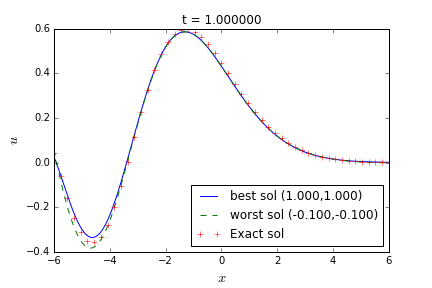
\includegraphics[scale=.375]{Fig1a.png}
\end{minipage}
\hfill
\begin{minipage}[t]{.5\linewidth}
	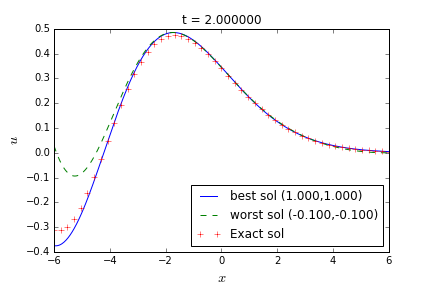
\includegraphics[scale=.375]{Fig1b.png}
\end{minipage}
\begin{minipage}[t]{.5\linewidth}
%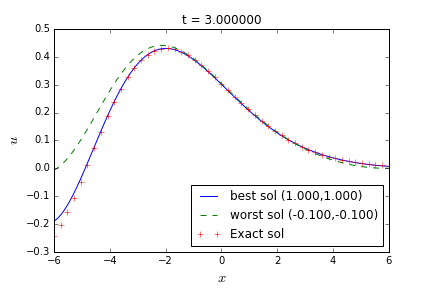
\includegraphics[scale=.5]{figures/FinalFigures/BessefirstTestsP0CorrectSnap3.png}
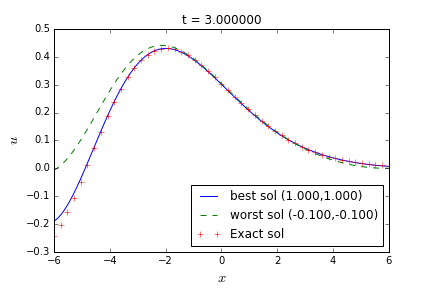
\includegraphics[scale=.375]{Fig1c.png}
\end{minipage}
\hfill
\begin{minipage}[t]{.5\linewidth}
%	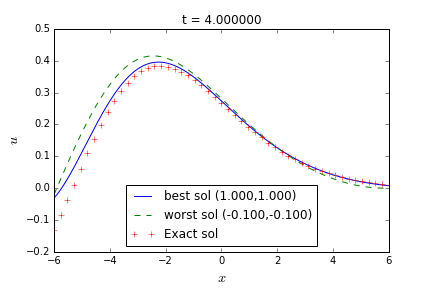
\includegraphics[scale=.5]{figures/FinalFigures/BessefirstTestsP0CorrectSnap4.png}
	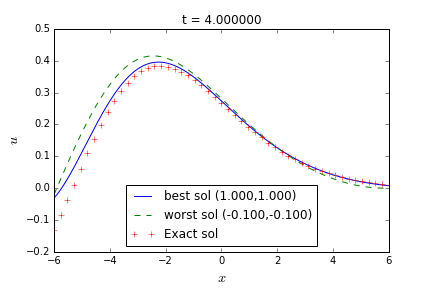
\includegraphics[scale=.375]{Fig1d.png}
\end{minipage}
\captionof{figure}{Best and worst solution compared with analytical solution, for the constant polynomial approximation \label{fig:firstTestsP0}}
\endgroup

\sisetup{round-mode=places}
\begin{center}
\begin{tabular}{c|c|S[round-precision=4,table-number-alignment =  left]}
	\multicolumn{1}{c|}{$c_L$}  & \multicolumn{1}{c|}{$c_R$} & \multicolumn{1}{r}{$e_{L2}$} \\
	\hline
	1.0 & 1.0 & 0.107543810109 \\
	1.0 & 10.0 & 0.109856882002 \\
	1.0 & 0.1 & 0.110879377847 \\
	1.0 & 0.0 & 0.111613324985 \\
	1.0 & -10.0 & 0.111708161825 \\
	1.0 & -0.1 & 0.112349327006 \\
	1.0 &  -1. & 0.113781032309 \\
	10.0 & 1.0 & 0.344703849892 \\
	10.0 & 0.1 & 0.345100899836 \\
	10.0 & 0.0 & 0.345208181531
\end{tabular}
\captionof{table}{Best results (smallest $e_{L2}$) for the constant polynomial approximation \label{tab:firstTestsP0}}
\end{center}

\deleted{
\indent It must be clear that our approach does not provide better transparent boundary conditions than the one proposed by \cite{besse2015}, what, as discussed in the introduction of this paper, is not the objective of the work developed here. Indeed, \cite{besse2015} derives TBCs for two discrete schemes, and the worst result among them, using the same $\Delta x $ and $\Delta t$ that we used here, presents an error $e_{L2} \approx 0.005$ for $t = 4$, while our best result has $e_{L2} \approx 0.1$ for the same instant. Nevertheless, considering that our main goal is the application of \deleted{the TBCs} \added{operators} to a domain decomposition method, we focus in minimizing the error due to the interface boundary conditions imposed in this kind of method, and not in the errors due to the external boundary conditions. For this same reason, we did not attempt to optimize the \added{operators in the role of} approximated TBCs (by finding the coefficients that provide the smallest error), and we performed tests only over a small set of possible coefficients, allowing us to observe the general behaviour of our approach. An optimization of the IBCs will be made in the next section, in the context of the domain decomposition methods.  } %deleted

\deleted{
\indent \deleted{As a conclusion of the work presented in this section, we can say that the boundary conditions proposed here work relatively well as TBCs, with a very simple implementation (without need, for example, of storing the solution of many previous time steps).} As a development of our approach, we also tested an approximation for $\lambda^2/s$ using a linear polynomial, but, although the increment in the complexity (including time derivative terms up to the second derivative, what requires the storage of previous computed solutions), it does not provide a better approximation for the TBCs, in comparison with the approximation using a constant polynomial.  } %deleted

\deleted{
\indent Therefore, in the sequel of this paper, we will continue using the \deleted{approximate TBCs given by the }operators $\Theta_i^{c}, \ i=1,2,3$, defined in \eqref{eq:appTBCP0}.  } %deleted